{\noindent\normalfont\bfseries\Large Appendices}

\appendix

\section{Angular distribution}
\label{sec:appendix:angular-distribution}

The transversity-basis moments of the 41 orthonormal angular functions defined in Eq.~\ref{eqn:vector_moments} are shown in Table~\ref{table:spd_mom_trans}. The orthonormal angular basis is constructed out of the spherical harmonics, \mbox{$Y^m_l \equiv Y^m_l (\thetal,\phi)$}
, and the reduced spherical harmonics, \mbox{${P^m_l \equiv \sqrt{2 \pi}Y^m_l(\thetak,0)}$}. The S, P and D-wave transversity amplitudes are denoted as $S^{\{L,R\}}$, $H^{\{L,R\}}_{\{0,\parallel,\perp\}}$ and $D^{\{L,R\}}_{\{0,\parallel,\perp\}}$, respectively.
\begin{table}[!tb]
\centering
\caption{The transversity-basis moments of the 41 orthonormal angular functions $f_i(\Omega)$ in Eq.~\ref{eqn:vector_moments}.}
\label{table:spd_mom_trans}
\resizebox{\textwidth}{!}{
\begin{tabular}{lccc} 
 $i$    &   $f_i(\Omega)$             & $\Gamma^{L, {\rm tr}}_i(\qsq)$ & $\eta^{L\to R}_i$  \\ \hline 
 1   &   $P^0_0 Y^0_0$     &  $\left[ \hzsq + \hpasq + \hpesq + \ssq + \dzsq + \dpasq + \dpesq\right]$ & + ($L \to R$)\\ 
 2   &   $P^0_1 Y^0_0$     &  $2\left[\frac{2}{\sqrt{5}} \rhzdz + \rshz + \sqrt{\frac{3}{5}}  \rel( H^L_\parallel D^{L\ast}_\parallel + H^L_\perp D^{L\ast}_\perp  )\right]$ & " \\ 
 3   &   $P^0_2 Y^0_0$     &  $\frac{\sqrt{5}}{7}$ (\dpasq + \dpesq) - $\frac{1}{\sqrt{5}}$ (\hpasq + \hpesq) + $\frac{2}{\sqrt{5}}$ \hzsq  + $\frac{10}{7\sqrt{5}}$ \dzsq + $2$ \rsdz & " \\  
 4   &   $P^0_3 Y^0_0$     &  $\frac{6}{\sqrt{35}} \left[ - \rel(H^L_\parallel D^{L\ast}_\parallel +  H^L_\perp D^{L\ast}_\perp)  + \sqrt{3} \rhzdz  \right]$ & "\\  
 5   &   $P^0_4 Y^0_0$     &  $\frac{2}{7} \left[ -2 (\dpasq + \dpesq) + 3 \dzsq \right] $ & "\\  
 6   &   $P^0_0 Y^0_2$     &  $\frac{1}{2 \sqrt{5}} \left[ (\dpasq + \dpesq) + (\hpasq + \hpesq) - 2 \ssq - 2 \dzsq - 2 \hzsq \right]$ & " \\  
 7   &   $P^0_1 Y^0_2$     &  $\left[ \frac{\sqrt{3}}{5} \rel(H^L_\parallel D^{L\ast}_\parallel  + H^L_\perp D^{L\ast}_\perp) - \frac{2}{\sqrt{5}} \rel(S^L H^{L\ast}_0)  - \frac{4}{5} \rel(H^L_0 D^{L\ast}_0)\right] $ & "  \\ 
 8   &   $P^0_2 Y^0_2$     &  $ \left[ \frac{1}{14} (\dpasq + \dpesq) - \frac{2}{7} \dzsq - \frac{1}{10} (\hpasq + \hpesq) - \frac{2}{5} \hzsq - \frac{2}{\sqrt{5}} \rsdz \right]$ & "  \\  
 9   &   $P^0_3 Y^0_2$     &  $ - \frac{3}{5 \sqrt{7}} \left[ \rel( H^L_\parallel D^{L \ast}_\parallel + H^L_\perp D^{L \ast}_\perp) + 2 \sqrt{3} \rel(H^L_0 D^{L \ast}_0 ) \right] $ & "\\ 
 10  &   $P^0_4 Y^0_2$     &  $ -\frac{2}{7 \sqrt{5}}  \left[ \dpasq + \dpesq + 3 \dzsq \right] $ & "  \\  
 11  &   $P^1_1 \sqrt{2}\rel(Y^1_2)$ &  $-\frac{3}{\sqrt{10}} \left[ \sqrt{\frac{2}{3}} \rel(H^L_\parallel S^{L \ast}) - \sqrt{\frac{2}{15}} \rel(H^L_\parallel D^{L \ast}_0  ) + \sqrt{\frac{2}{5}} \rel(D^L_\parallel H^{L \ast}_0 ) \right] $  & "\\  
 12  &   $P^1_2 \sqrt{2}\rel(Y^1_2)$ &  $-\frac{3}{5} \left[ \rel( H^L_\parallel H^{L \ast}_0)  + \sqrt{\frac{5}{3}} \rel (D^L_\parallel S^{L \ast})  + \frac{5}{7 \sqrt{3}} \rel(D^L_\parallel D^{L\ast}_0) \right] $ & " \\  
 13  &   $P^1_3 \sqrt{2}\rel(Y^1_2)$ &  $-\frac{6}{5 \sqrt{14}} \left[2 \rel(D^L_\parallel H^{L\ast}_0)  + \sqrt{3} \rel(H^L_\parallel D^{L\ast}_0 ) \right] $ & " \\  
 14  &   $P^1_4 \sqrt{2}\rel(Y^1_2)$ &  $- \frac{6}{7\sqrt{2}} \rel(D^L_\parallel D^{L\ast}_0)$  & " \\  
 15  &   $P^1_1 \sqrt{2}\img(Y^1_2)$ &  $3 \left[ \frac{1}{\sqrt{15}} \img(H^L_\perp S^{L\ast}) + \frac{1}{5} \img(D^L_\perp H^{L\ast}_0) - \frac{1}{5 \sqrt{3}}  \img(H^L_\perp D^{L\ast}_0) \right]  $  & " \\  
 16  &   $P^1_2 \sqrt{2}\img(Y^1_2)$ &  $ 3\left[ \frac{1}{7 \sqrt{3}} \img(D^L_\perp D^{L\ast}_0)  + \frac{1}{5} \img(H^L_\perp H^{L\ast}_0)  + \frac{1}{\sqrt{15}} \img(D^L_\perp S^{L\ast})   \right] $  & " \\
 17  &   $P^1_3 \sqrt{2}\img(Y^1_2)$ &  $\frac{6}{5 \sqrt{14}} \left[ 2 \img(D^L_\perp H^{L\ast}_0)  + \sqrt{3} \img(H^L_\perp D^{L\ast}_0) \right]  $   & " \\  
 18  &   $P^1_4 \sqrt{2}\img(Y^1_2)$ &  $\frac{6}{7\sqrt{2}} \img(D^L_\perp D^{L\ast}_0)$  & " \\  
 19  &   $P^0_0 \sqrt{2}\rel(Y^2_2)$ &  $-\frac{3}{2\sqrt{15}} \left[ (\hpasq - \hpesq) + (\dpasq - \dpesq) \right] $  & " \\  
 20  &   $P^0_1 \sqrt{2}\rel(Y^2_2)$ &  $-\frac{3}{5} \left[ \rel(H^L_\parallel D^{L\ast}_\parallel)   - \rel(D^L_\perp H^{L\ast}_\perp) \right] $  & " \\  
 21  &   $P^0_2 \sqrt{2}\rel(Y^2_2)$ &  $\frac{\sqrt{3}}{2} \left[ - \frac{1}{7} (\dpasq - \dpesq)   + \frac{1}{5} ( \hpasq - \hpesq ) \right] $  & " \\  
 22  &   $P^0_3 \sqrt{2}\rel(Y^2_2)$ &  $\frac{3}{5} \sqrt{ \frac{3}{7}} \left[ \rel(H^L_\parallel D^{L\ast}_\parallel)   - \rel(D^L_\perp H^{L\ast}_\perp) \right] $  & " \\ 
 23  &   $P^0_4 \sqrt{2}\rel(Y^2_2)$ &  $\frac{2}{7} \sqrt{ \frac{3}{5}}  (\dpasq - \dpesq) $ & " \\  
 24  &   $P^0_0 \sqrt{2}\img(Y^2_2)$ &  $\sqrt{\frac{3}{5}} \left[ \img(H^L_\perp H^{L\ast}_\parallel) + \img(D^L_\perp D^{L\ast}_\parallel) \right] $   & " \\  
 25  &   $P^0_1 \sqrt{2}\img(Y^2_2)$ &  $\frac{3}{5} \img(  H^L_\perp D^{L\ast}_\parallel +  D^L_\perp H^{L\ast}_\parallel )  $  & " \\ 
 26  &   $P^0_2 \sqrt{2}\img(Y^2_2)$ &  $ \sqrt{3} \left[\frac{1}{7} \img(D^L_\perp D^{L\ast}_\parallel)   - \frac{1}{5} \img(H^L_\perp H^{L\ast}_\parallel)\right] $  & " \\
 27  &   $P^0_3 \sqrt{2}\img(Y^2_2)$ &  $-\frac{3}{5} \sqrt{ \frac{3}{7}}  \img(D^L_\perp H^{L\ast}_\parallel + H^L_\perp D^{L\ast}_\parallel)  $  & " \\
 28  &   $P^0_4 \sqrt{2}\img(Y^2_2)$ &  $-\frac{4}{7} \sqrt{\frac{3}{5}}  \img(D^L_\perp D^{L\ast}_\parallel) $   & " \\ 
 29  &   $P^0_0 Y^0_1$     &  $-\sqrt{3}\left[ \rel(H^L_\perp H^{L\ast}_\parallel) + \rel(D^L_\perp D^{L\ast}_\parallel) \right]$  & - ($L \to R$) \\
 30  &   $P^0_1 Y^0_1$     &  $-\frac{3}{\sqrt{5}} \rel( H^L_\perp D^{L\ast}_\parallel + H^L_\parallel D^{L\ast}_\perp ) $ & " \\
 31  &   $P^0_2 Y^0_1$     &  $-\frac{3}{\sqrt{15}} \left[ \frac{5}{7} \rel(D^L_\perp D^{L\ast}_\parallel) - \rel(H^L_\perp H^{L\ast}_\parallel)  \right]$ & " \\
 32  &   $P^0_3 Y^0_1$     &  $\frac{9}{\sqrt{105}}  \rel(H^L_\perp D^{L\ast}_\parallel  + H^L_\parallel D^{L\ast}_\perp ) $ & " \\
 33  &   $P^0_4 Y^0_1$     &  $\frac{4\sqrt{3}}{7} \rel(D^L_\perp D^{L\ast}_\parallel)$  & " \\
 34  &   $P^1_1 \sqrt{2}\rel(Y^1_1)$   & $\sqrt{\frac{3}{5}} \left[ \sqrt{5} \rel(H^L_\perp S^{L \ast})  + \sqrt{3} \rel(D^L_\perp H^{L\ast}_0)  - \rel(H^L_\perp D^{L \ast}_0) \right]$  & " \\
 35  &   $P^1_2 \sqrt{2}\rel(Y^1_1)$   & $ 3 \left[ \frac{1}{\sqrt{5}} \rel(H^L_\perp H^{L \ast}_0)  + \frac{1}{\sqrt{3}} \rel(D^L_\perp S^{L\ast})  + \frac{5}{21} \sqrt{\frac{3}{5}} \rel(D^L_\perp D^{L \ast}_0 ) \right] $  & " \\
 36  &   $P^1_3 \sqrt{2}\rel(Y^1_1)$   & $ \frac{6}{\sqrt{70}} \left[ 2 \rel(D^L_\perp H^{L \ast}_0)  + \sqrt{3} \rel(H^L_\perp D^{L\ast}_0) \right]$  & " \\
 37  &   $P^1_4 \sqrt{2}\rel(Y^1_1)$   & $\frac{3 \sqrt{10}}{7} \rel(D^L_\perp D^{L \ast}_0 ) $  & " \\
 38  &   $P^1_1 \sqrt{2}\img(Y^1_1)$   & $-\sqrt{\frac{3}{5}} \left[ \sqrt{5} \img ( H^L_\parallel S^{L\ast}) + \sqrt{3} \img(D^L_\parallel H^{L \ast}_0) - \img(H^L_\parallel D^{L \ast}_0)  \right]  $  & " \\
 39  &   $P^1_2 \sqrt{2}\img(Y^1_1)$   & $ -\sqrt{\frac{3}{5}} \left[ \sqrt{3} \img(H^L_\parallel H^{L \ast}_0)  + \sqrt{5} \img(D^L_\parallel S^{L\ast})  + \frac{5}{7} \img(D^L_\parallel D^{L \ast}_0 )\right] $  & " \\
 40  &   $P^1_3 \sqrt{2}\img(Y^1_1)$   & $ -6\sqrt{\frac{1}{70}}\left[ 2\img(D^L_\parallel H^{L \ast}_0)  + \sqrt{3} \img(H^L_\parallel D^{L\ast}_0)\right]$   & " \\
 41  &   $P^1_4 \sqrt{2}\img(Y^1_1)$   & $-\frac{3}{7} \sqrt{10} \img(D^L_\parallel D^{L\ast}_0) $  & " \\
\end{tabular}

}
\end{table}

\section{Agreement between data and simulation}
\label{sec:appendix:data-mc}

\subsection{PID resampling}
\label{sec:appendix:data-mc:pid}

\begin{figure}[!tb]
 \centering
 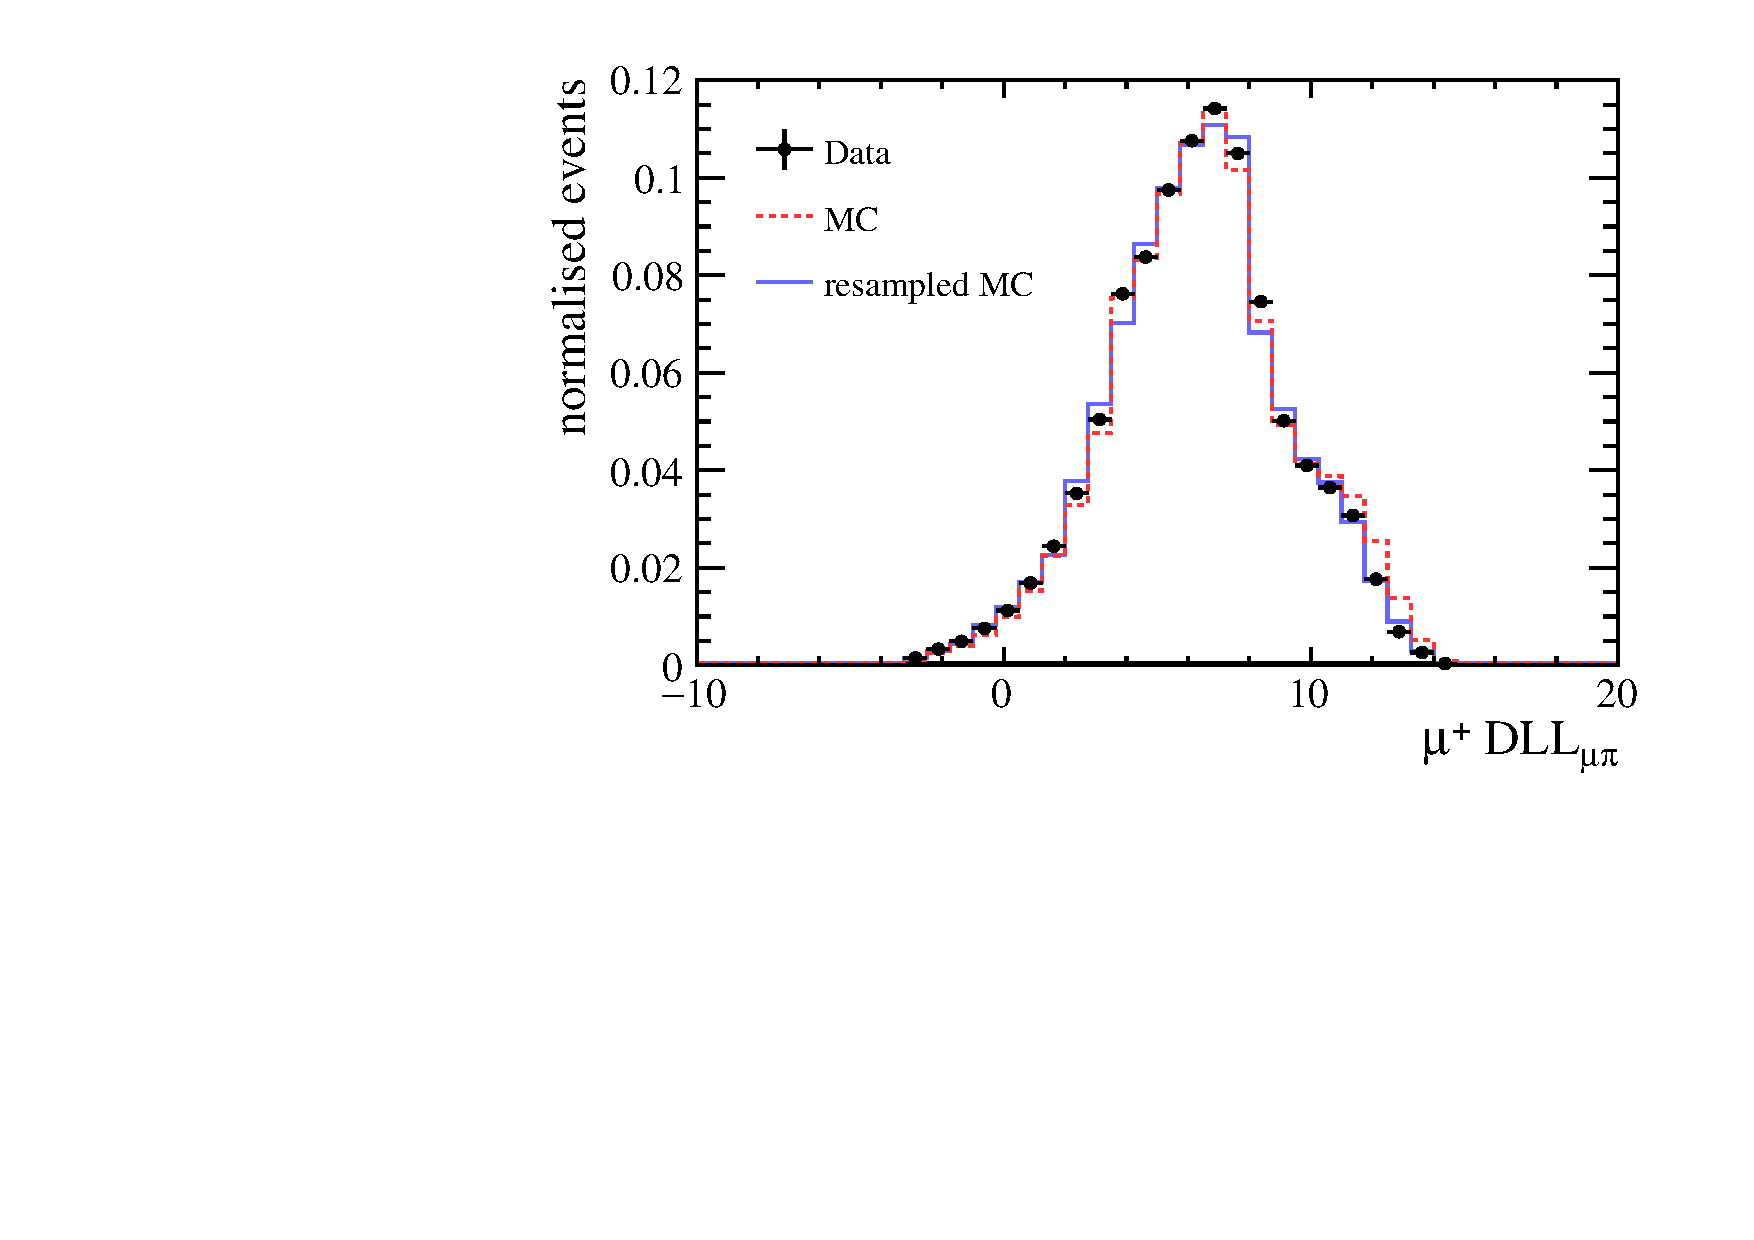
\includegraphics[width=0.49\textwidth]{figs/kpimm/data-mc/resampling/Muplus_PIDmu.pdf}
 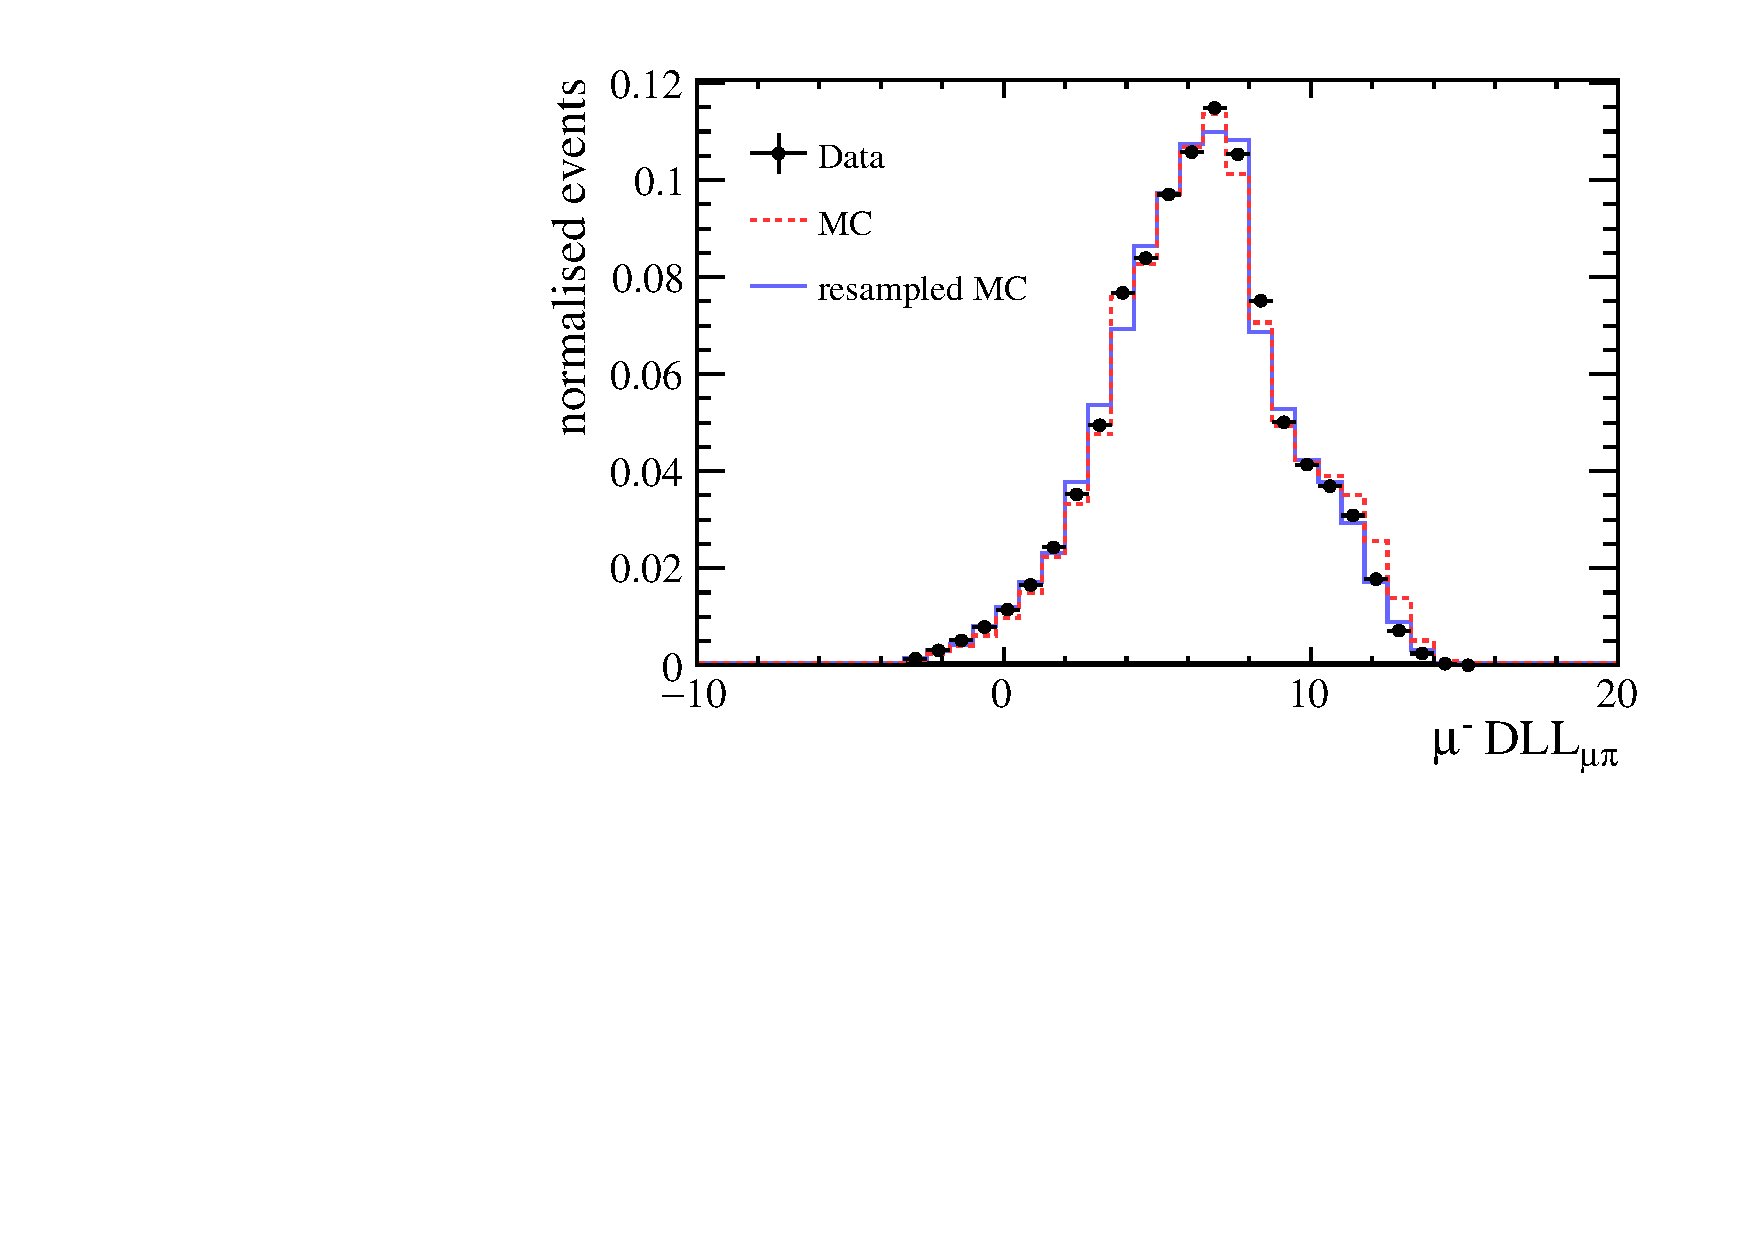
\includegraphics[width=0.49\textwidth]{figs/kpimm/data-mc/resampling/Muminus_PIDmu.pdf}
 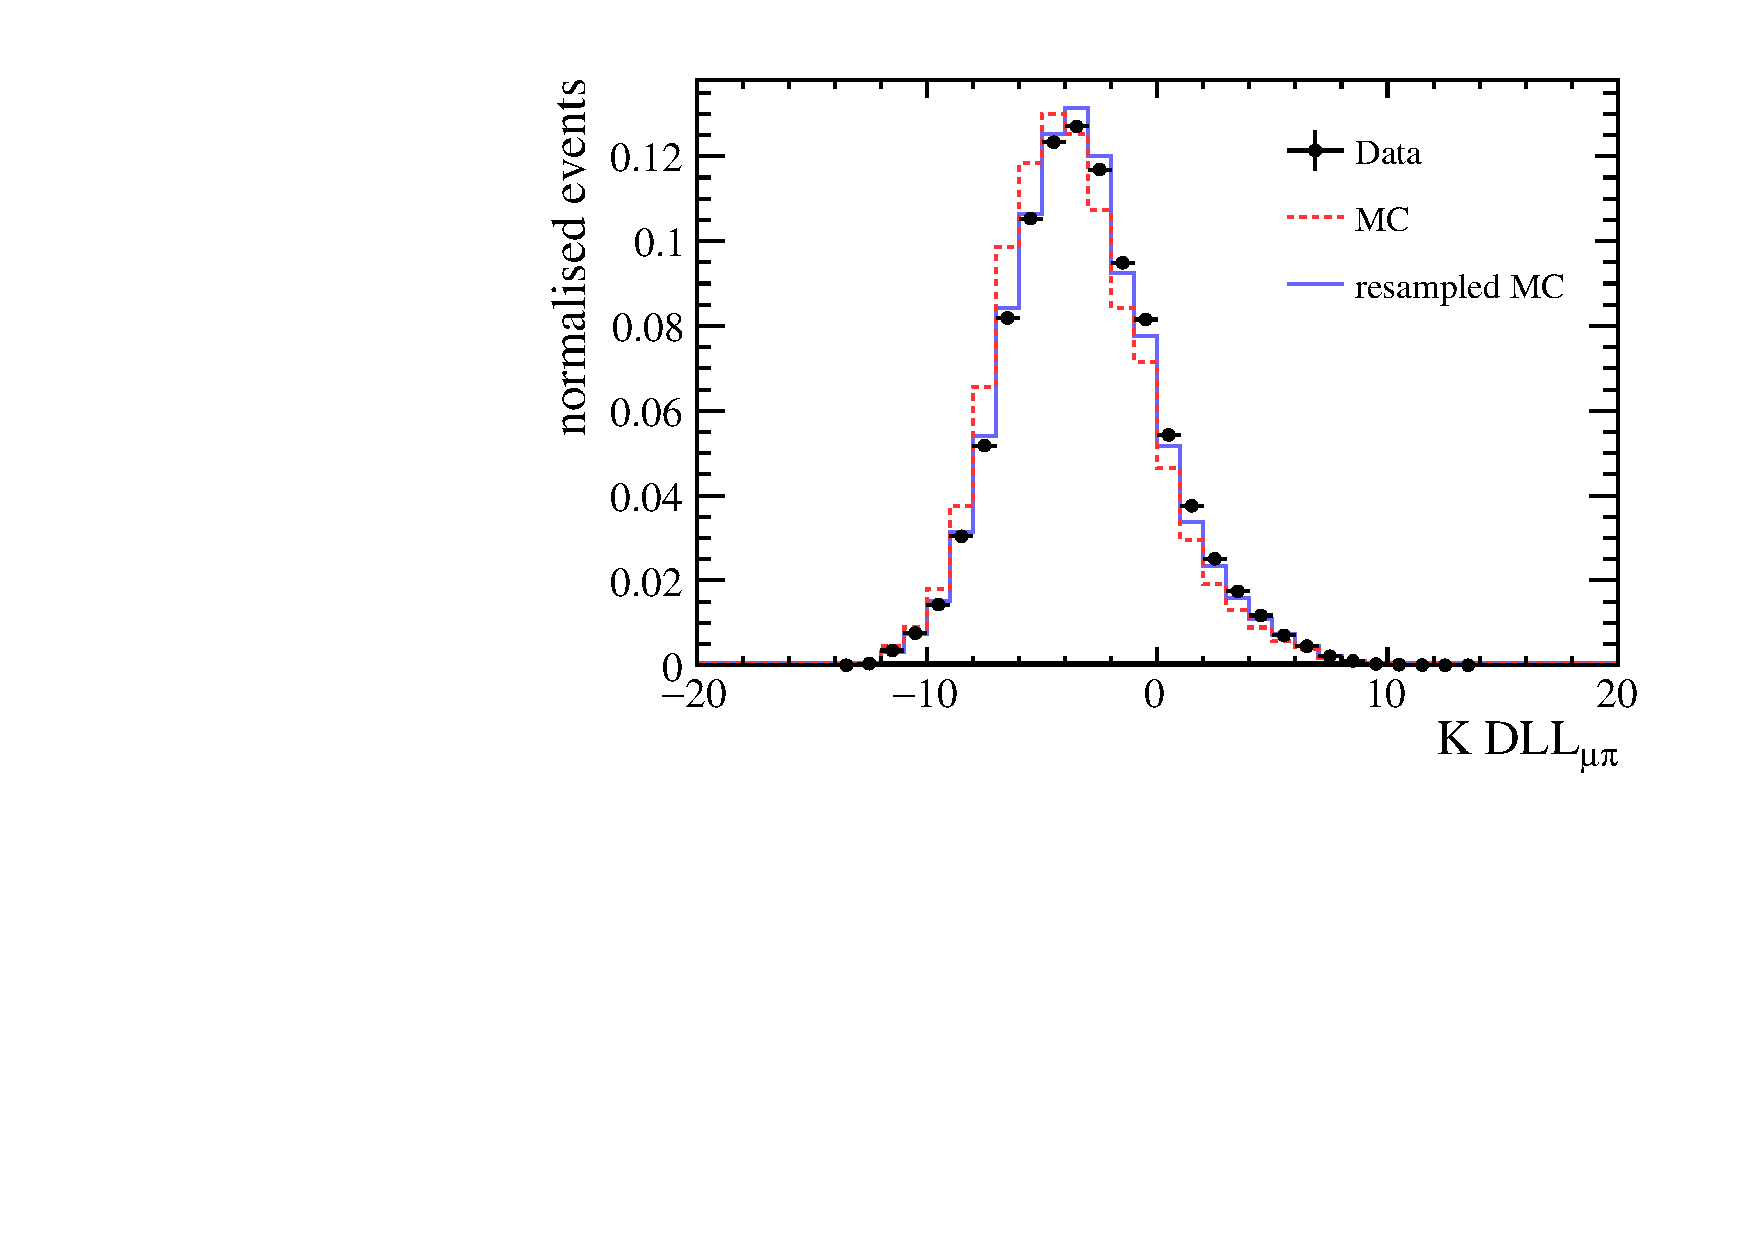
\includegraphics[width=0.49\textwidth]{figs/kpimm/data-mc/resampling/K_PIDmu.pdf}
 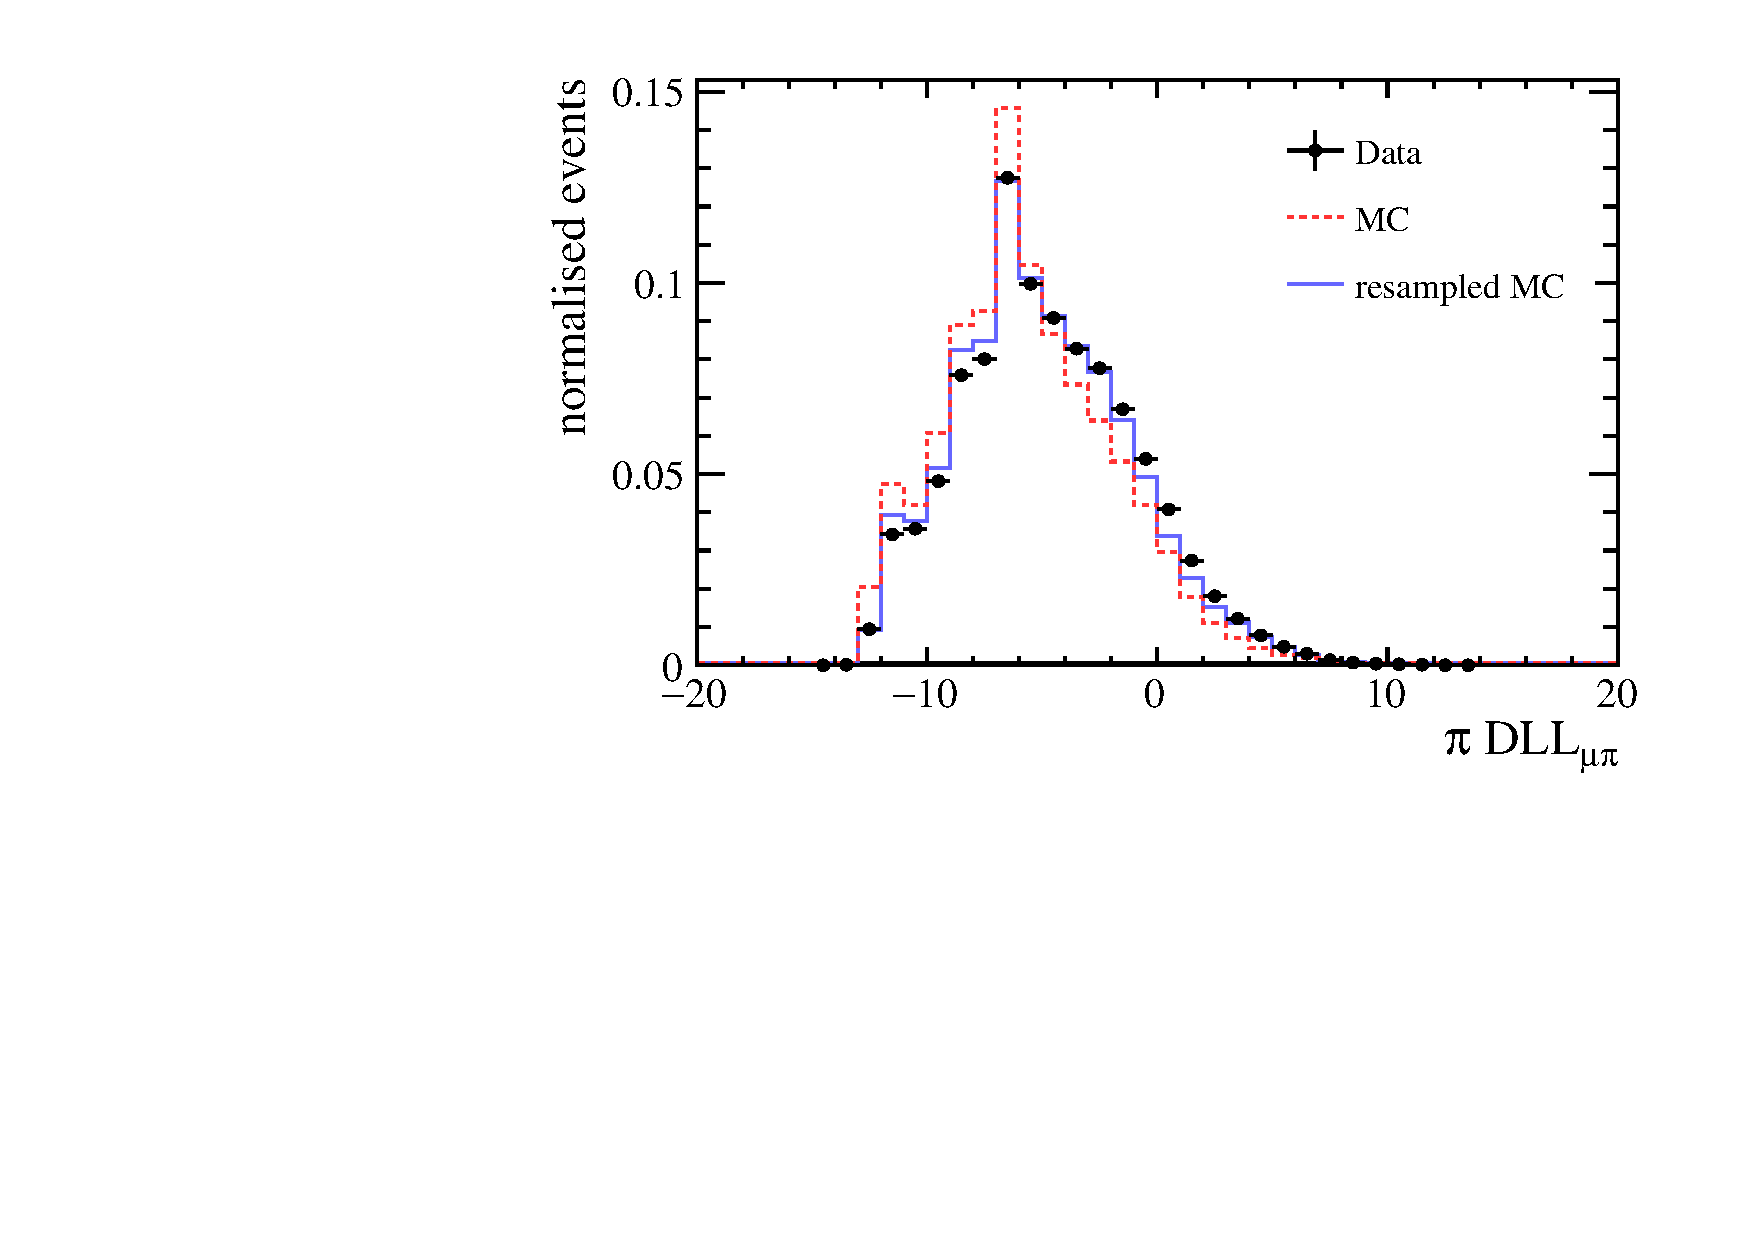
\includegraphics[width=0.49\textwidth]{figs/kpimm/data-mc/resampling/Pi_PIDmu.pdf}
 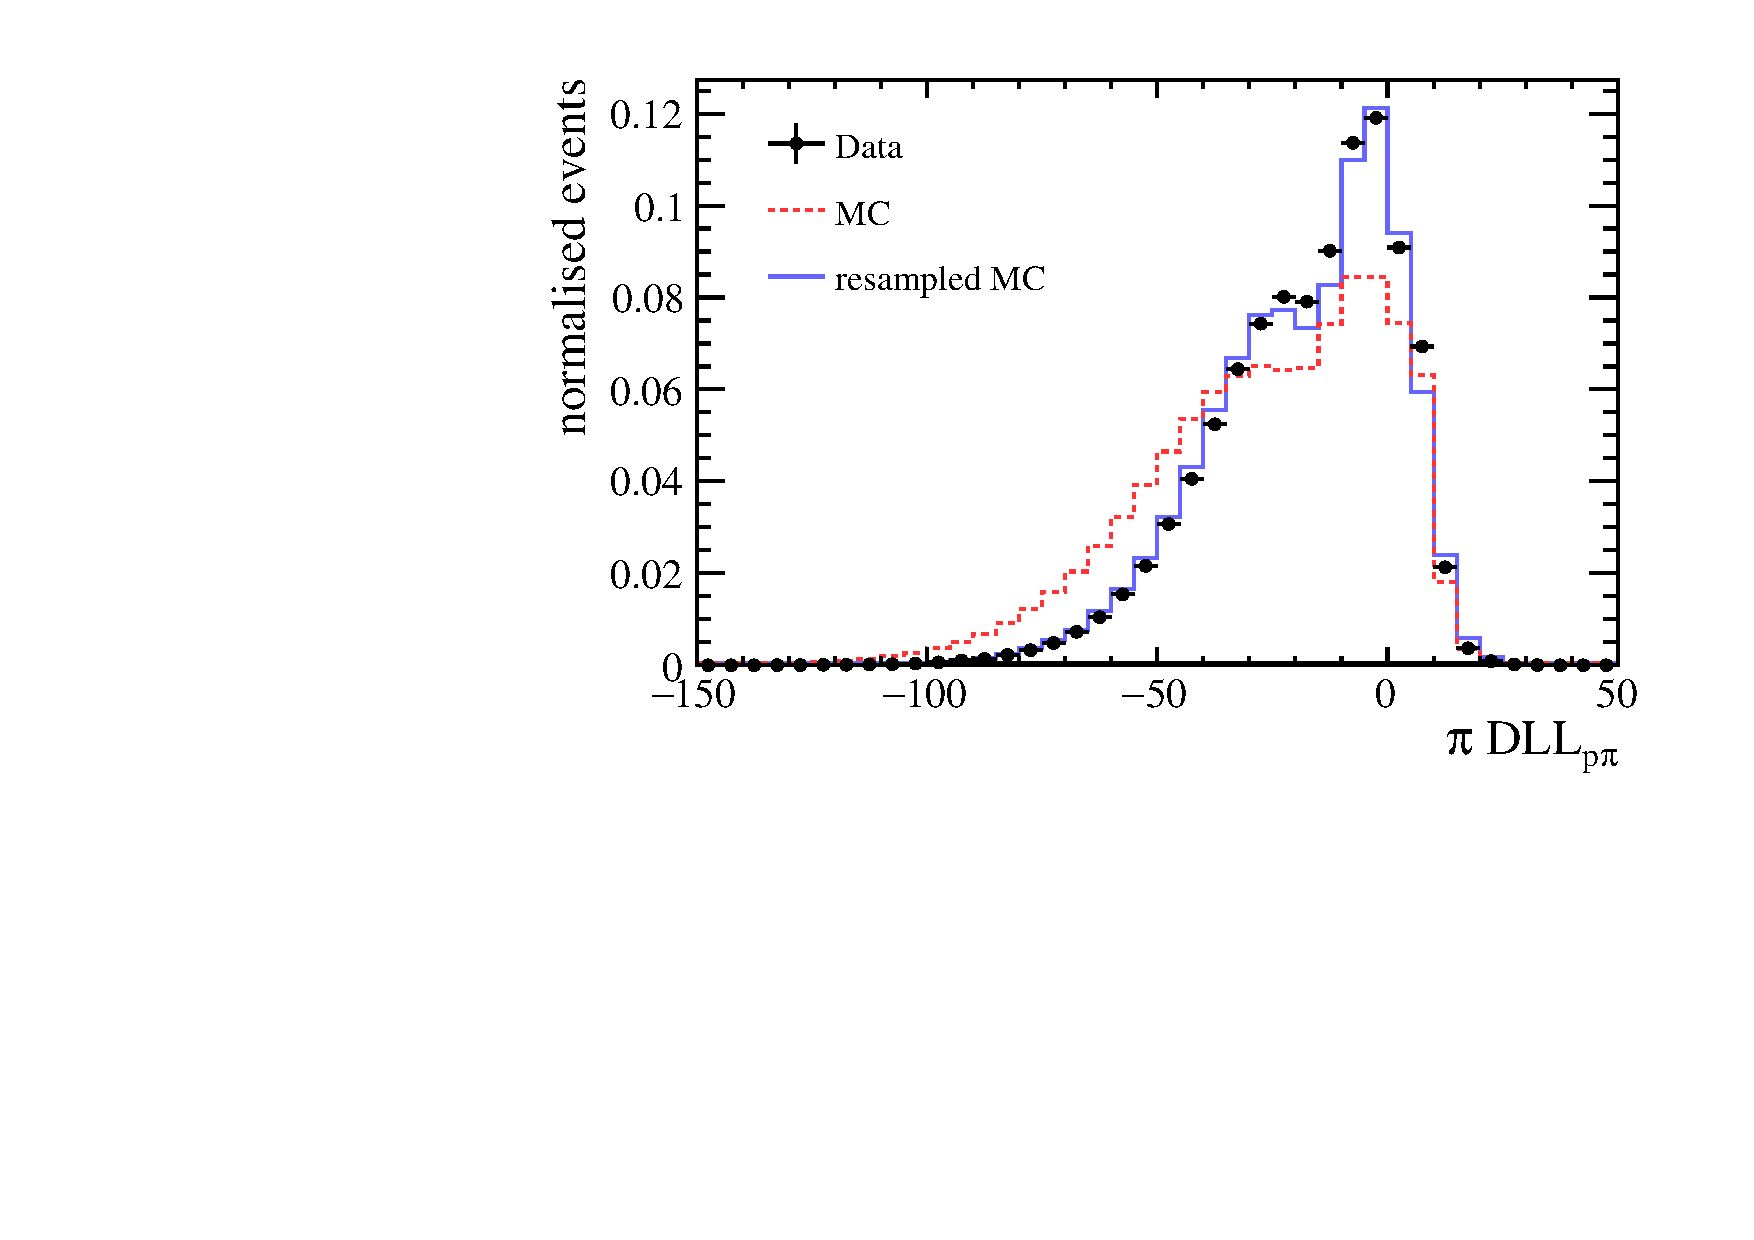
\includegraphics[width=0.49\textwidth]{figs/kpimm/data-mc/resampling/Pi_PIDp.pdf}
 \caption{Data-simulation agreement for the PID variables used in the selection of \BdToKpimm. The black data points show the distributions for sWeighted \BdToJPsiKst candidates in data. The red dashed histograms show the nominal distribution for simulated \BdToJPsiKst candidates. The blue histograms show the distribution for simulated \BdToJPsiKst candidates after the resampling procedure.}
\label{fig:kpimm:data-mc:pid}
\end{figure}

\section{The \kpimm invariant mass distribution}
\label{sec:appendix:massfits}

Figure~\ref{fig:massfit:bins} show the fits to the \mkpimm distribution in each of the \qsq bins used for the differential branching fraction measurement.
 
\begin{figure}[!tb]
\centering
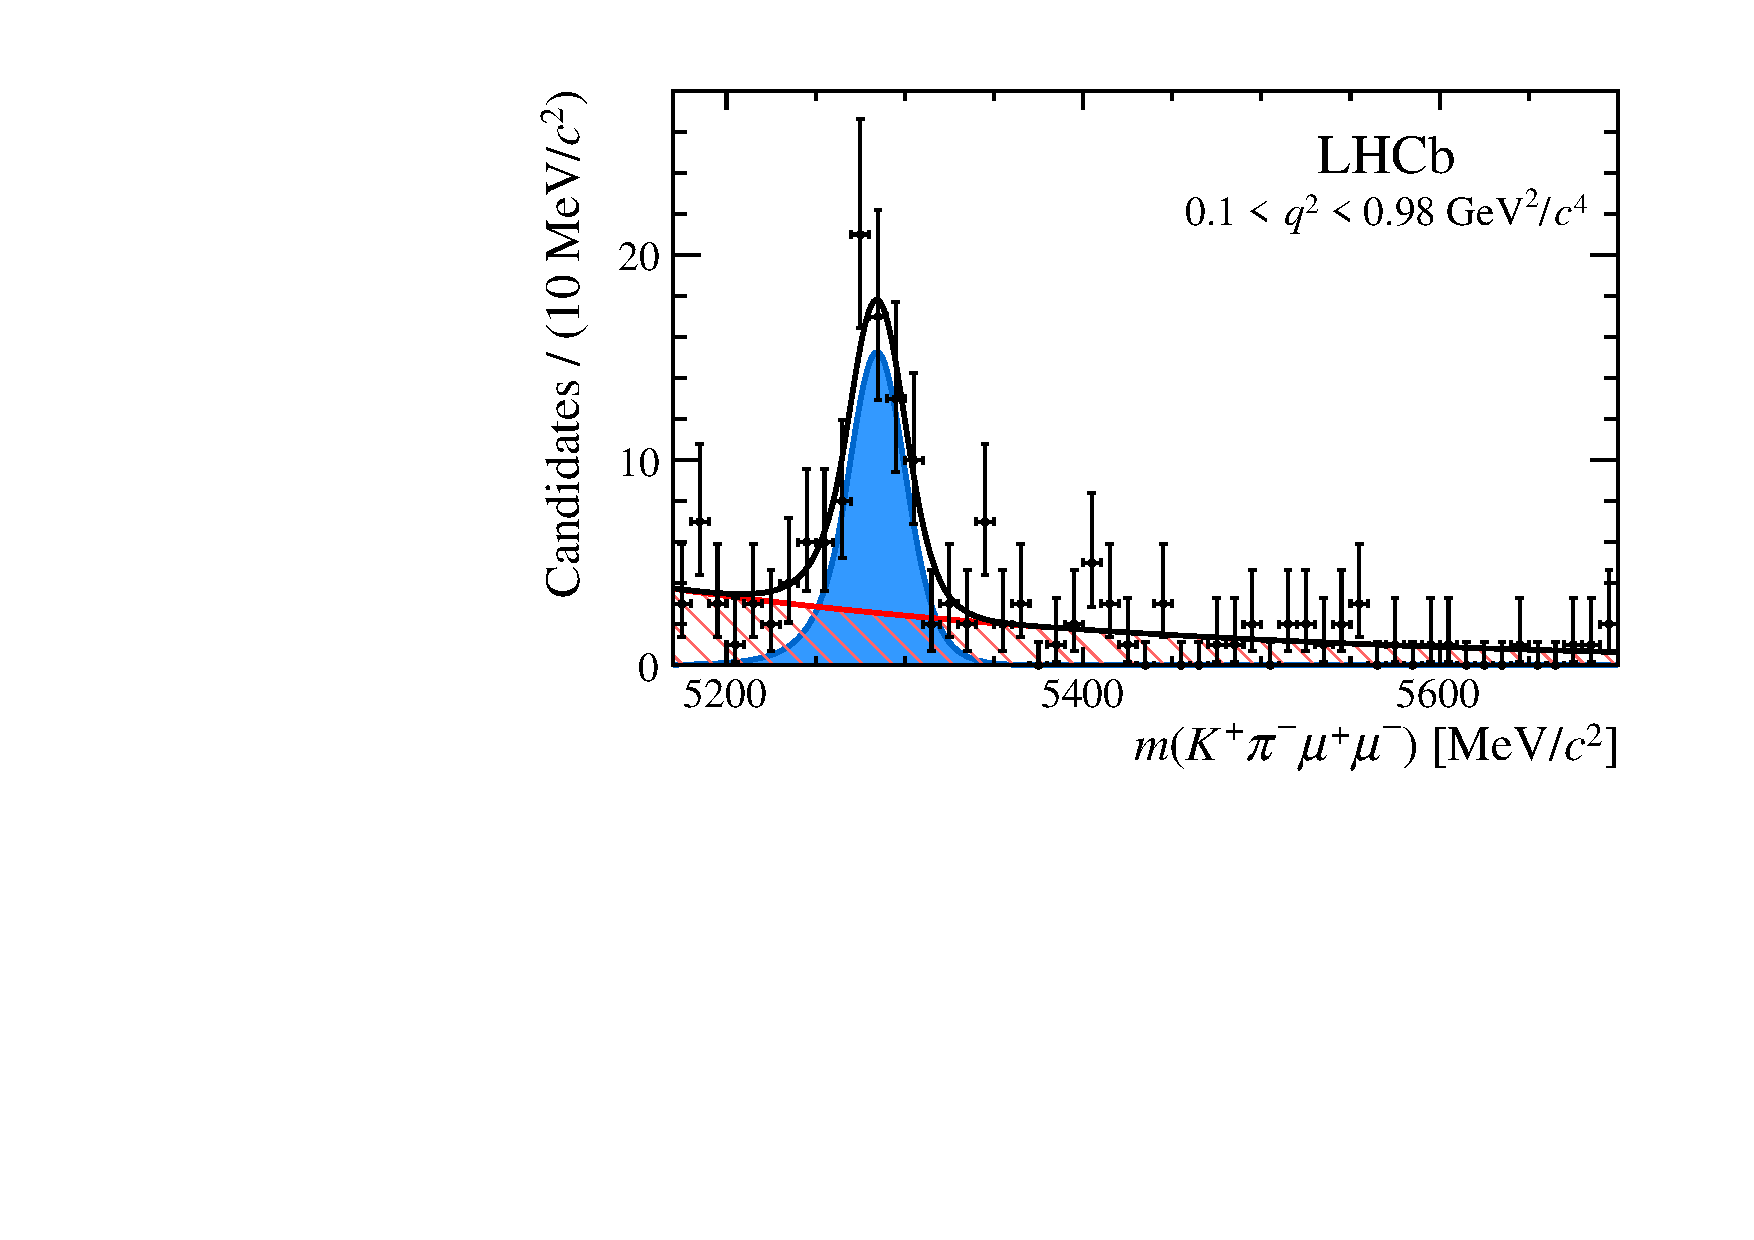
\includegraphics[width=0.48\linewidth]{figs/kpimm/massfit/fitKpimumu_q2_0p1_0p98.pdf}
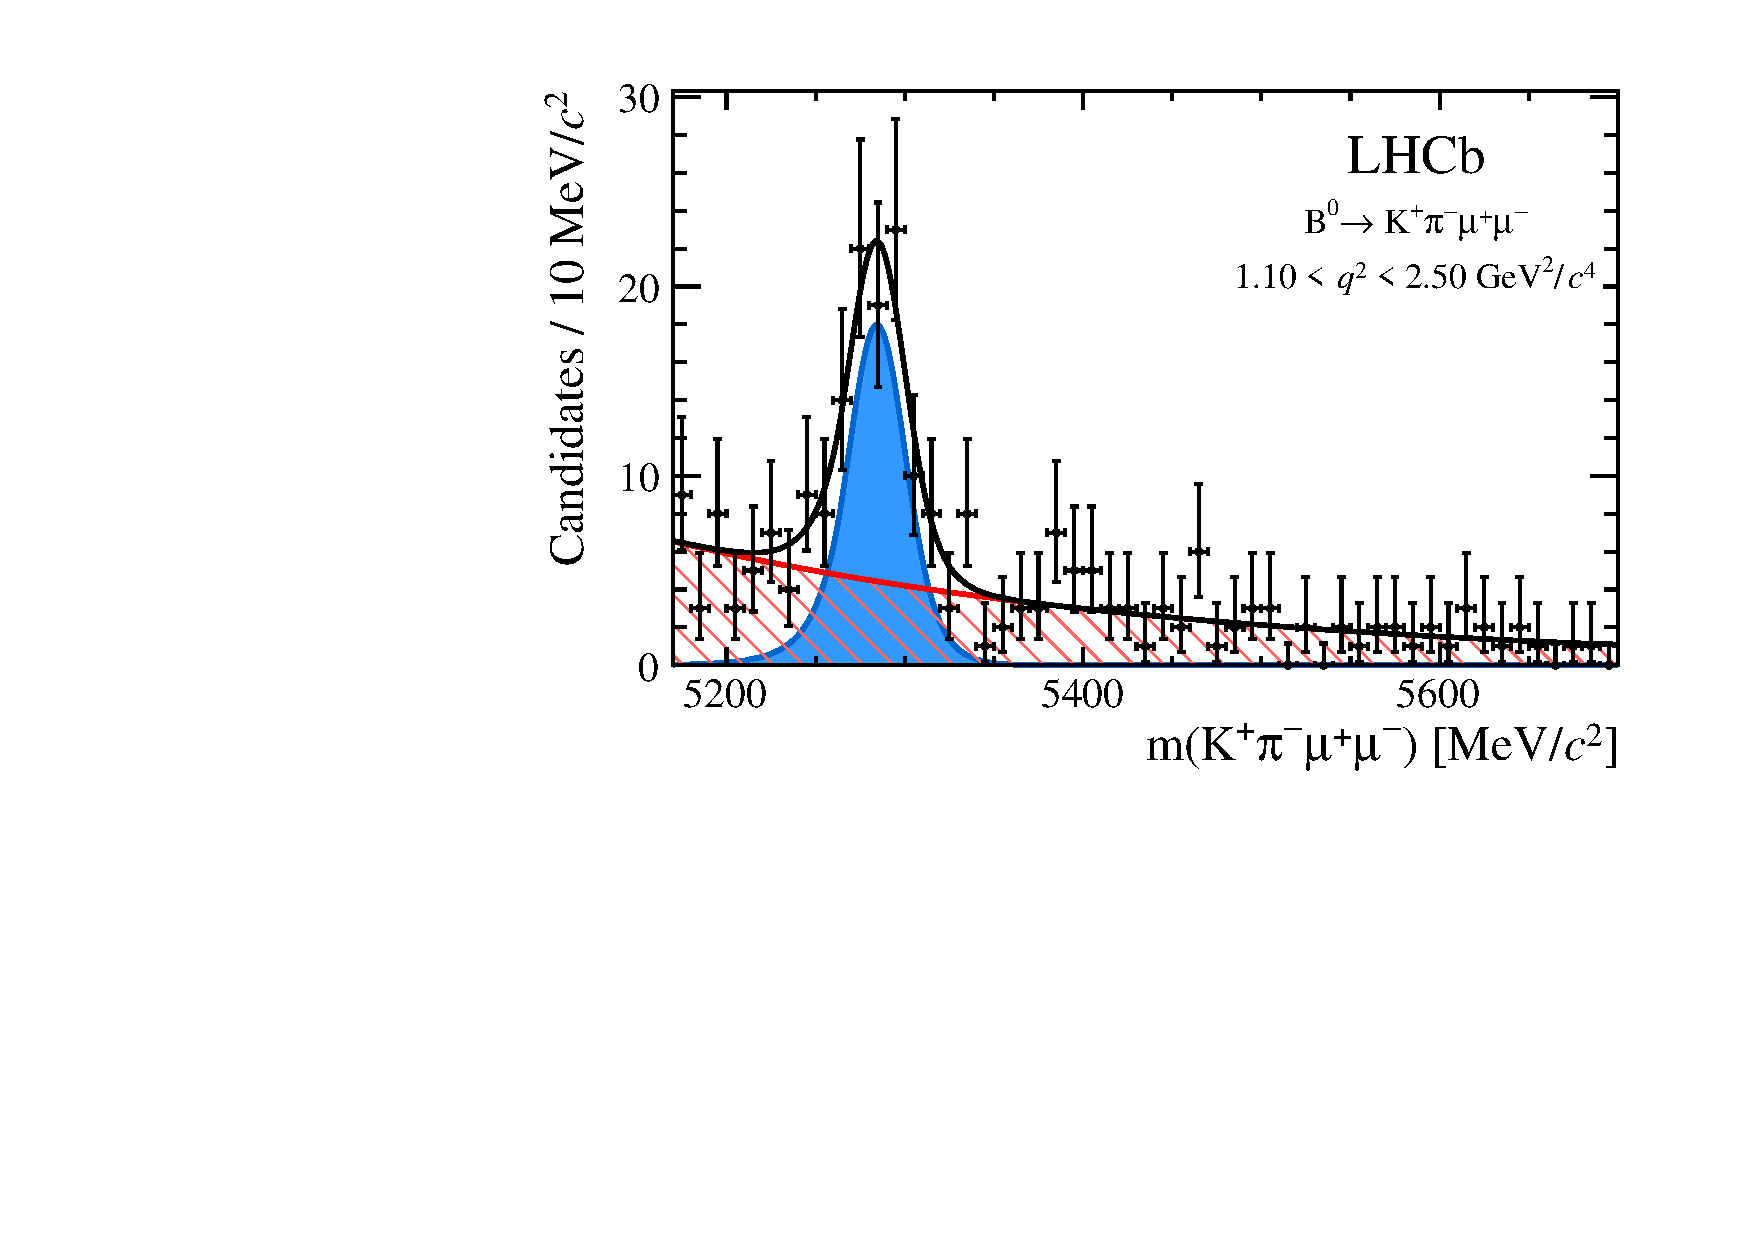
\includegraphics[width=0.48\linewidth]{figs/kpimm/massfit/fitKpimumu_q2_1p1_2p5.pdf}
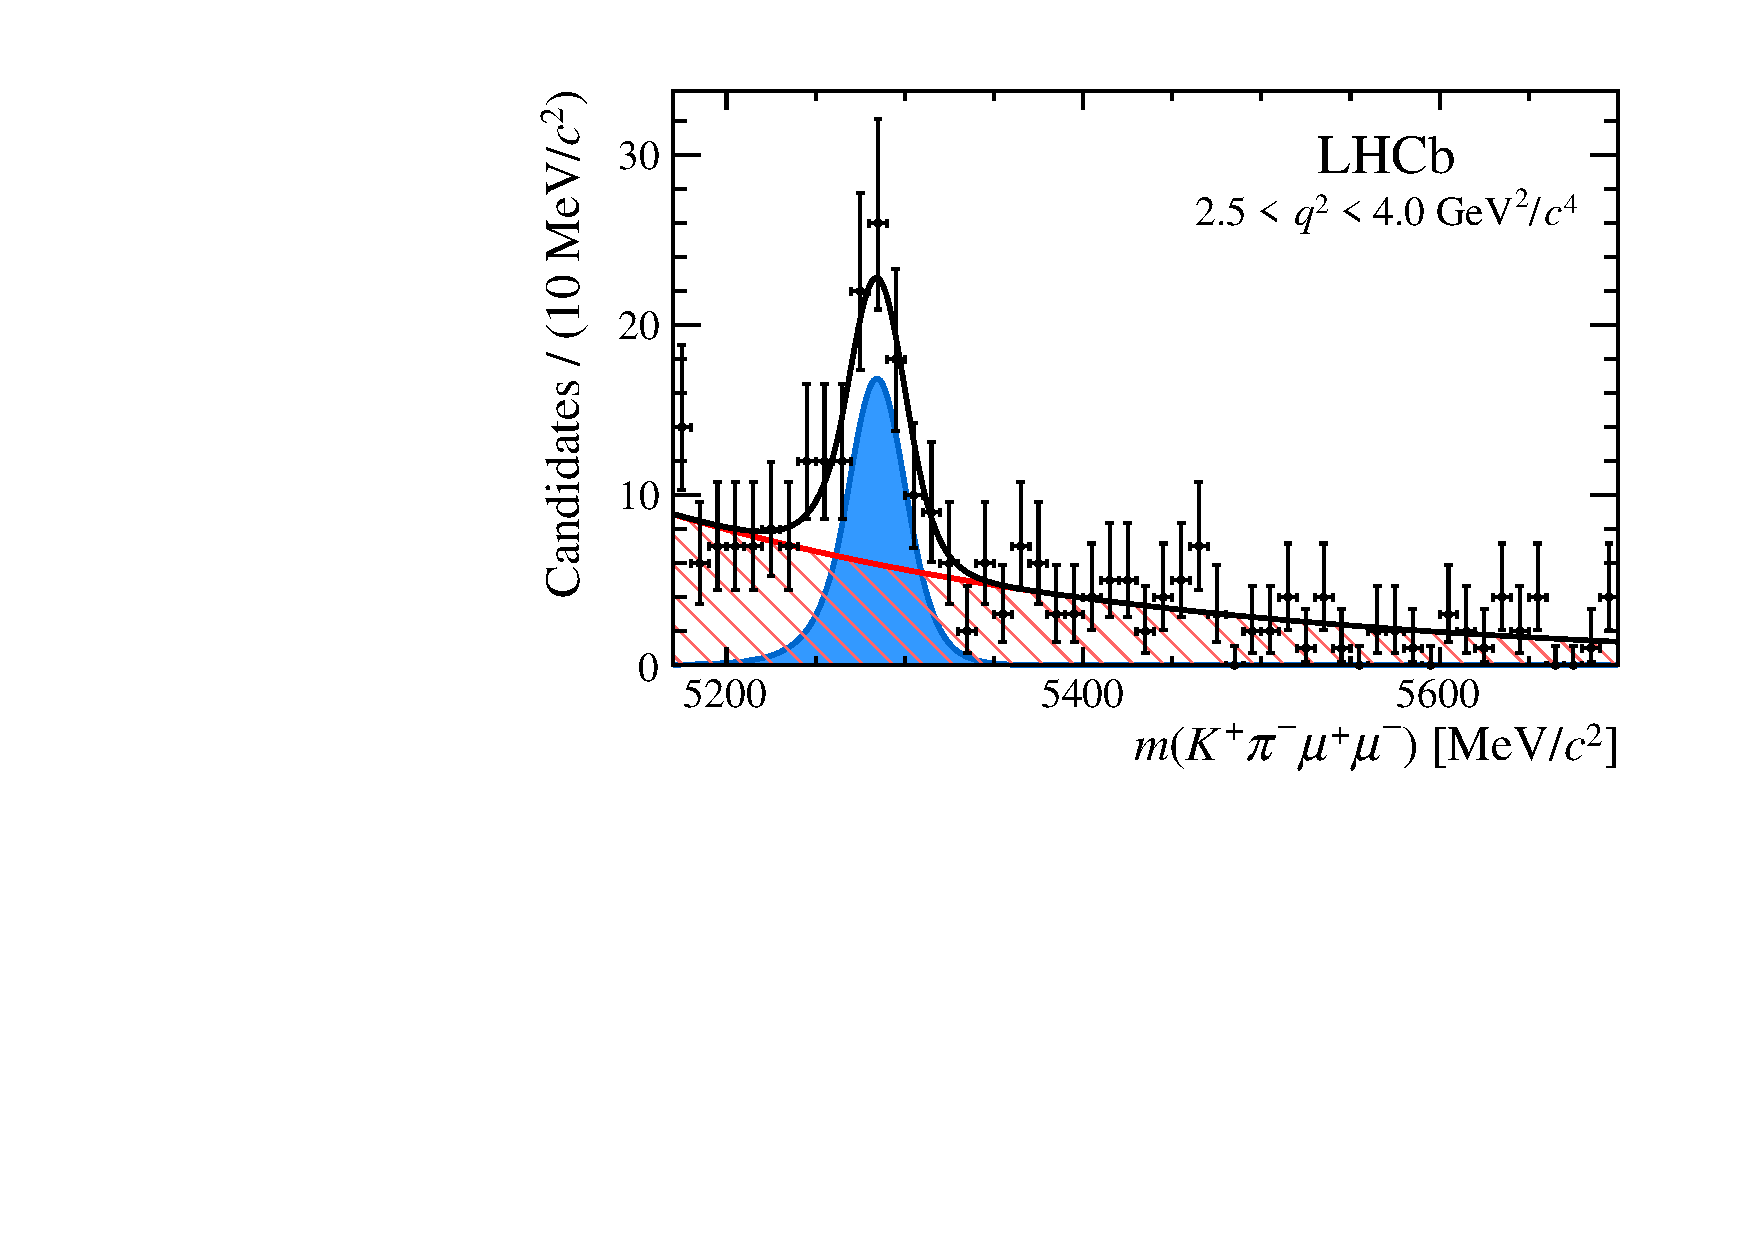
\includegraphics[width=0.48\linewidth]{figs/kpimm/massfit/fitKpimumu_q2_2p5_4p0.pdf}
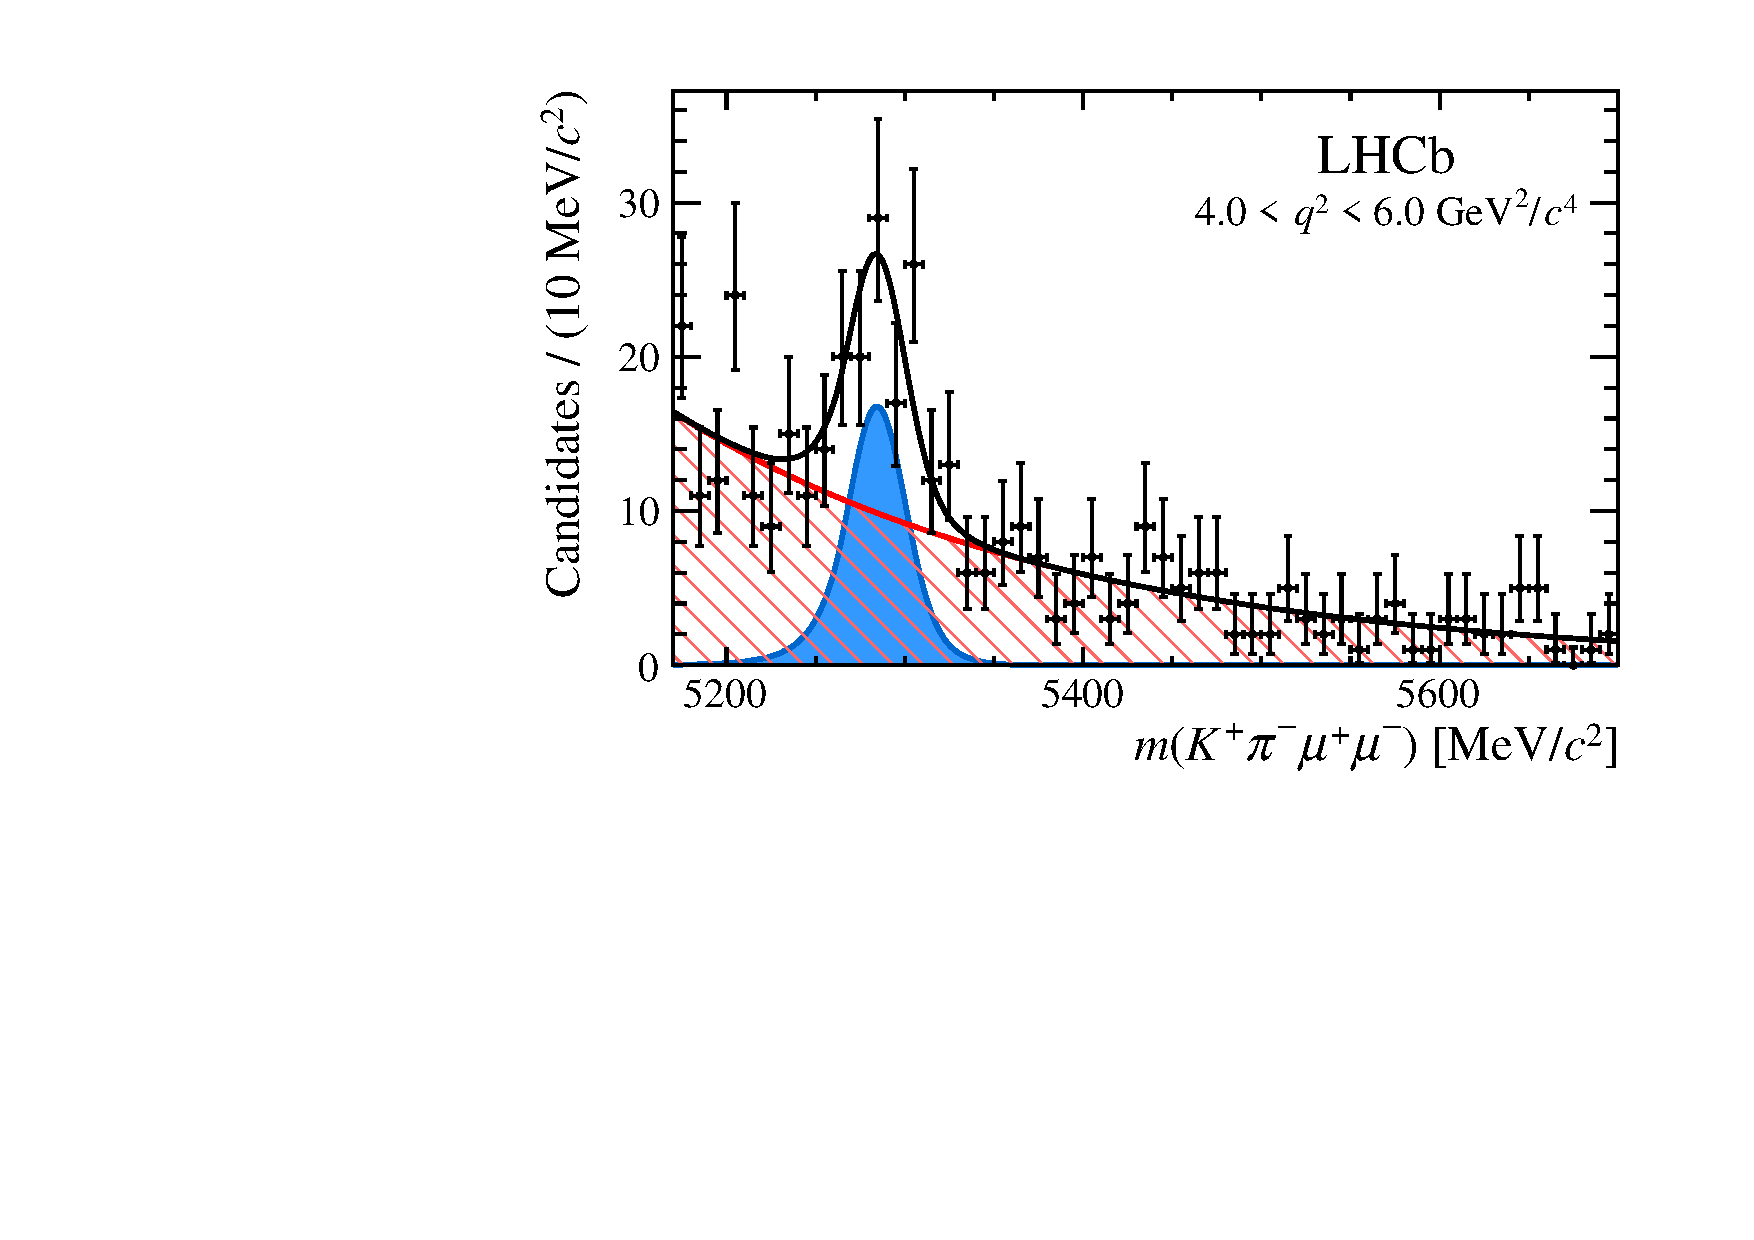
\includegraphics[width=0.48\linewidth]{figs/kpimm/massfit/fitKpimumu_q2_4p0_6p0.pdf}
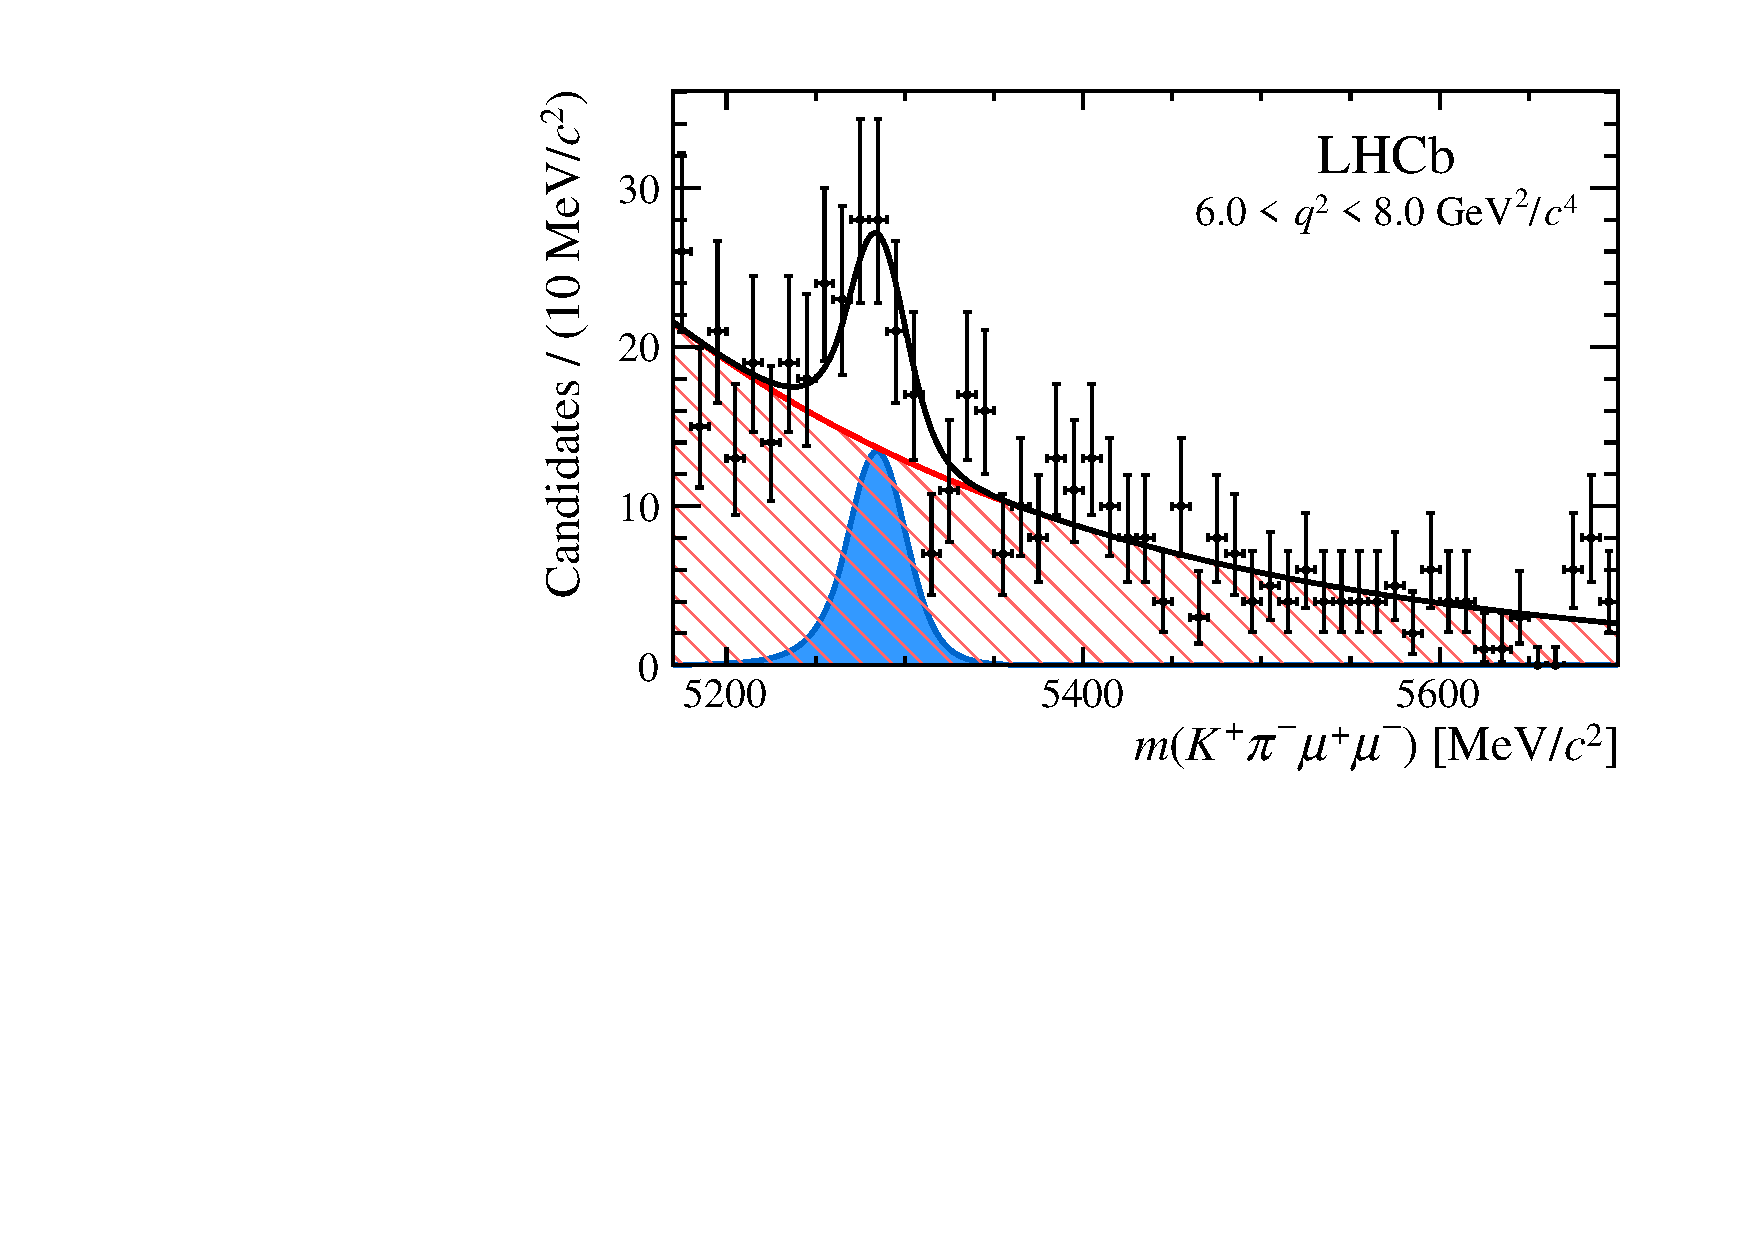
\includegraphics[width=0.48\linewidth]{figs/kpimm/massfit/fitKpimumu_q2_6p0_8p0.pdf}
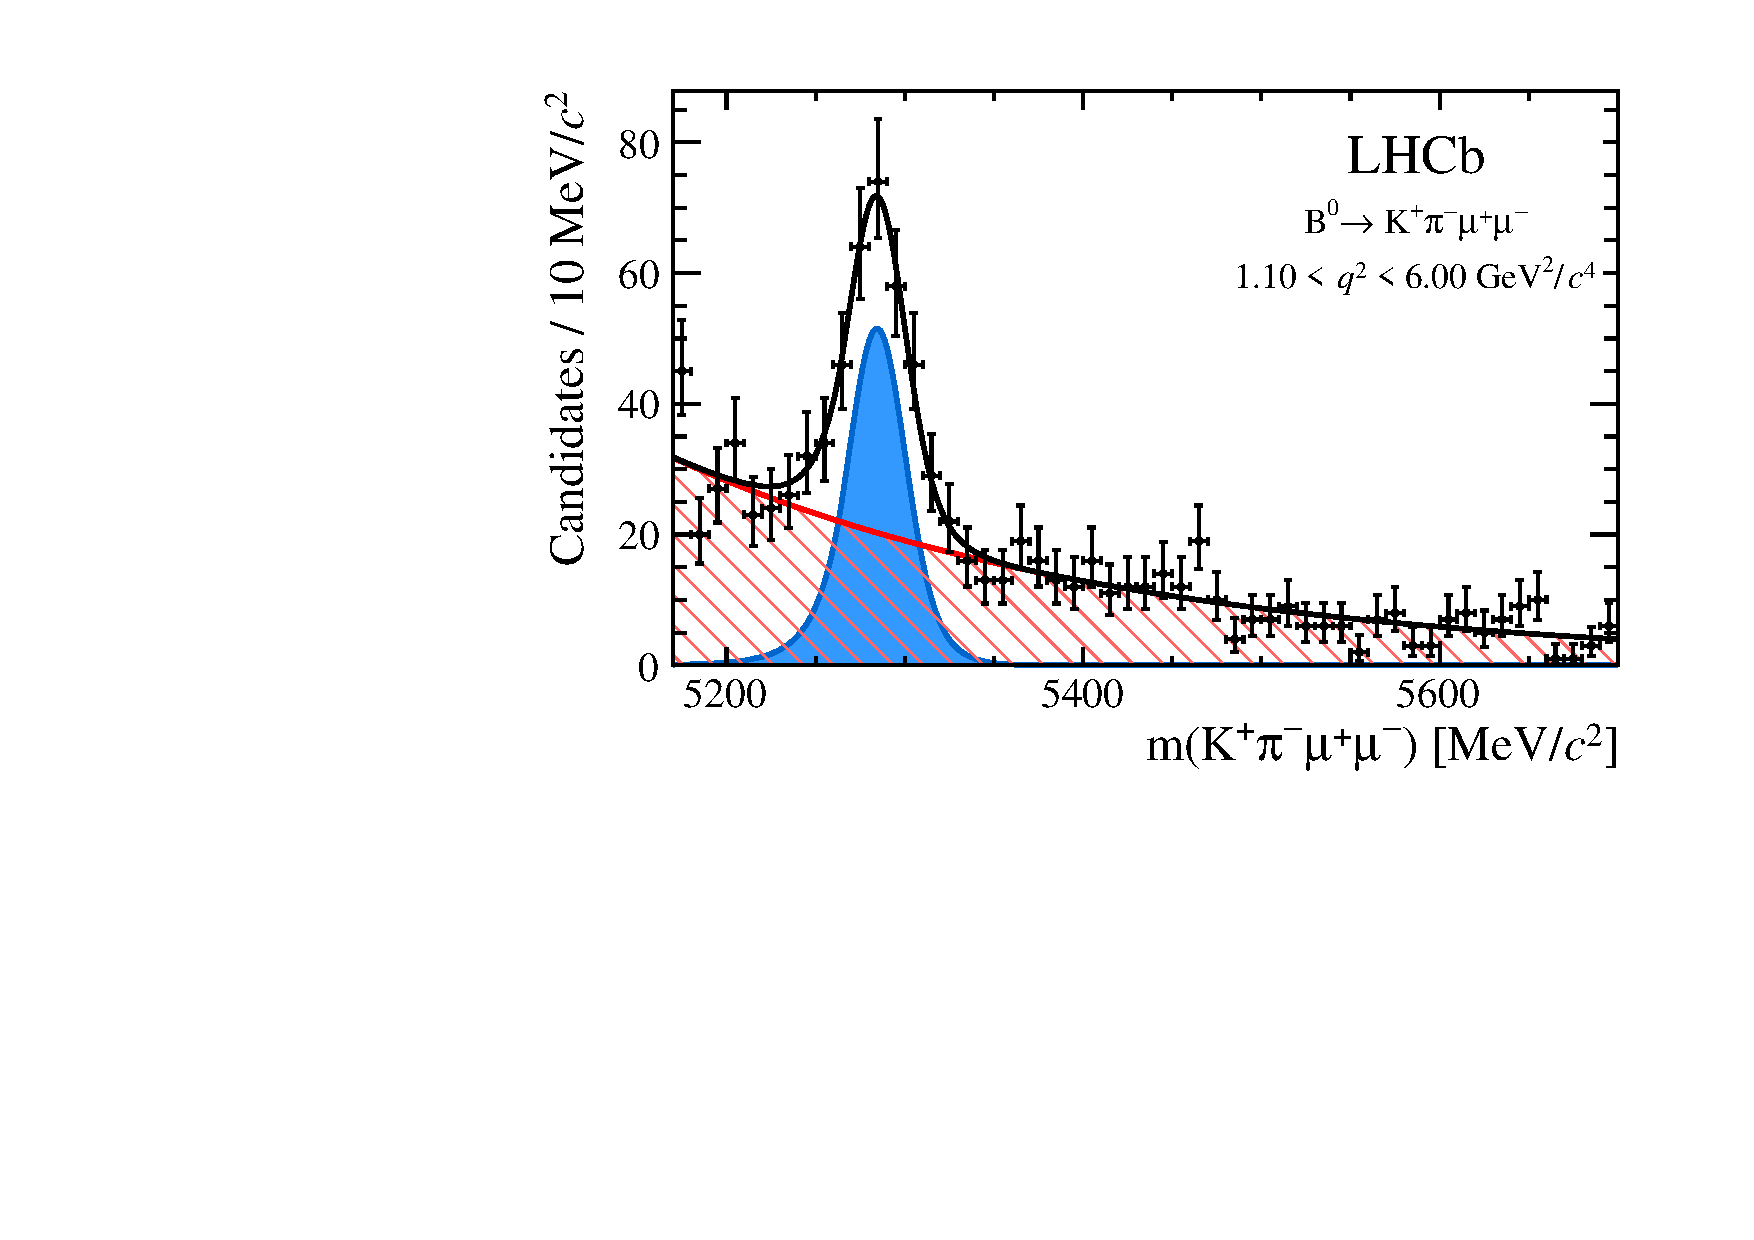
\includegraphics[width=0.48\linewidth]{figs/kpimm/massfit/fitKpimumu_q2_1p1_6p0.pdf}
 
\caption{Invariant mass \mkpimm for the signal decay \BdToKpimm in  each of the \qsq bins used for the differential branching fraction measurement. The solid black line represents the total fitted function.  The individual components of the signal (blue shaded area) and combinatorial background (red hatched area) are also shown.}
\label{fig:massfit:bins}
\end{figure}